\usepackage{tikz}
\usepackage{xstring}

% Aquí van todas las figuras en TikZ, hay que asignarlas un numero para poder cambiar todas a la vez.

\newcommand{\figura}[1]{
	\IfEqCase{#1}{
	% PARTE I %
		{hipervisor1}{\figurahipA}
		{hipervisor2}{\figurahipB}
		{hipervisor2real}{\figurahipBfin}
		{hardware}{\figuraHard}
		{sohost1}{\figuraSO}
		{sohost2}{\figuraSOsimpl}
		{hipervisor}{\fbox{\textcolor{red}{ESTA FIGURA HAY QUE HACERLA}}}
		{maqinavirtual}{\fbox{\textcolor{red}{ESTA FIGURA HAY QUE HACERLA}}}
		{virtualizacionnat}{\fbox{\textcolor{red}{ESTA FIGURA HAY QUE HACERLA}}}
		{virtualizacionhost}{\fbox{\textcolor{red}{ESTA FIGURA HAY QUE HACERLA}}}
		{vmware}{\fbox{\parbox{70mm}{\textcolor{red}{ESTA FIGURA HAY QUE HACERLA\\ ES COMO LA ÚLTIMA PERO LAS VM ESTAN EL EL SERVIDOR}}}}
	% PARTE II %
		{3}{\pizarra}
	}[\PackageError{figura}{Figura no declarada: #1}{}]
}


% Aqui se añaden las figuras %
\newcommand{\figurahipA}{
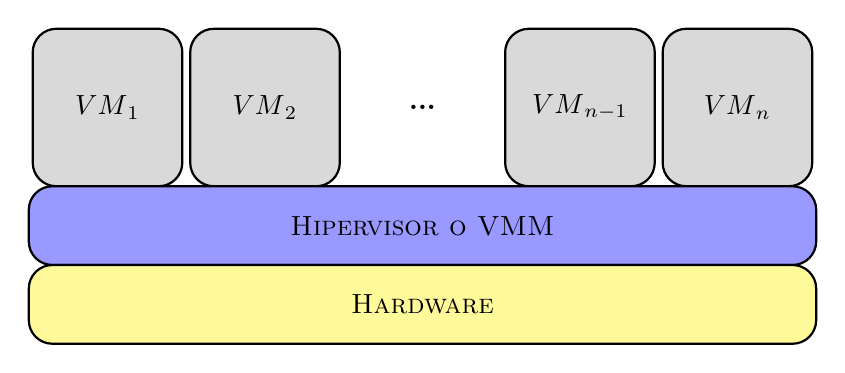
\begin{tikzpicture}
	\draw[rounded corners=3mm, fill=gray!30, thick] (0.05,2) rectangle (1.95,4);
	\draw[rounded corners=3mm, fill=gray!30, thick] (2.05,2) rectangle (3.95,4);
	\draw[rounded corners=3mm, fill=gray!30, thick] (6.05,2) rectangle (7.95,4);
	\draw[rounded corners=3mm, fill=gray!30, thick] (8.05,2) rectangle (9.95,4);
	\draw[rounded corners=3mm, fill={blue!40}, thick] (0,1) rectangle (10,2); 
	\draw[rounded corners=3mm, fill=yellow!40, thick] (0,0) rectangle (10,1); 

	\node at (1,3) {${VM}_1$};
	\node at (3,3) {${VM}_2$};
	\node at (5,3) {\textbf{...}};
	\node at (7,3) {${VM}_{n-1}$};
	\node at (9,3) {${VM}_n$};
	\node at (5,1.5) {\textsc{Hipervisor o VMM}};
	\node at (5,0.5) {\textsc{Hardware}};
\end{tikzpicture}
}

\newcommand{\figurahipB}{
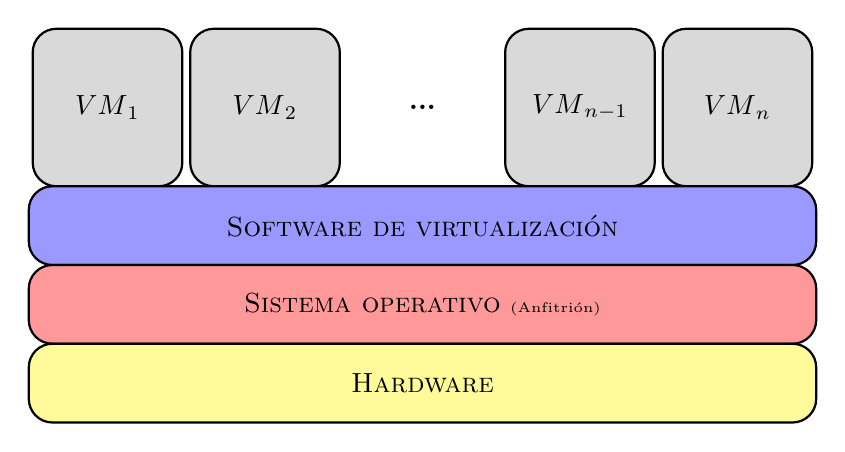
\begin{tikzpicture}
	\draw[rounded corners=3mm, fill=gray!30, thick] (0.05,3) rectangle (1.95,5);
	\draw[rounded corners=3mm, fill=gray!30, thick] (2.05,3) rectangle (3.95,5);
	\draw[rounded corners=3mm, fill=gray!30, thick] (6.05,3) rectangle (7.95,5);
	\draw[rounded corners=3mm, fill=gray!30, thick] (8.05,3) rectangle (9.95,5);
	\draw[rounded corners=3mm, fill={blue!40}, thick] (0,2) rectangle (10,3);
	\draw[rounded corners=3mm, fill={red!40}, thick] (0,1) rectangle (10,2); 
	\draw[rounded corners=3mm, fill=yellow!40, thick] (0,0) rectangle (10,1); 

	\node at (1,4) {${VM}_1$};
	\node at (3,4) {${VM}_2$};
	\node at (5,4) {\textbf{...}};
	\node at (7,4) {${VM}_{n-1}$};
	\node at (9,4) {${VM}_n$};
	\node at (5,2.5) {\textsc{Software de virtualización}};
	\node at (5,1.5) {\textsc{Sistema operativo} {\tiny (Anfitrión)}};
	\node at (5,0.5) {\textsc{Hardware}};
\end{tikzpicture}
}

\newcommand{\figurahipBfin}{
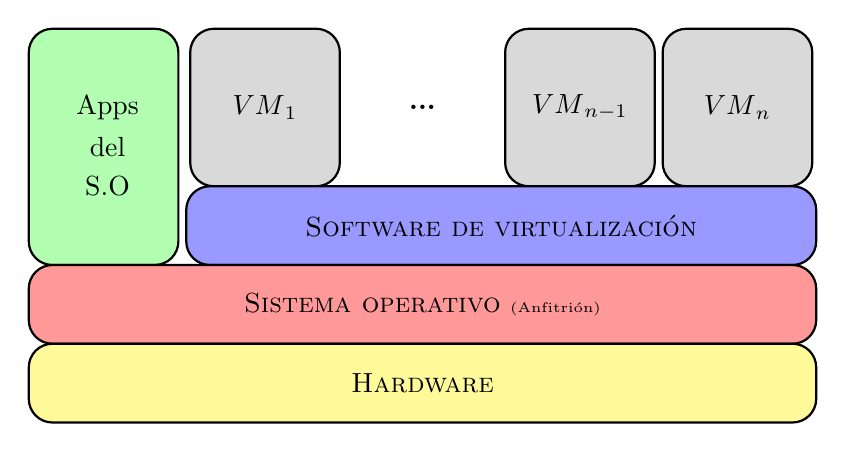
\begin{tikzpicture}
	\draw[rounded corners=3mm, fill=green!30, thick] (0,2) rectangle (1.90,5);
	\draw[rounded corners=3mm, fill=gray!30, thick] (2.05,3) rectangle (3.95,5);
	\draw[rounded corners=3mm, fill=gray!30, thick] (6.05,3) rectangle (7.95,5);
	\draw[rounded corners=3mm, fill=gray!30, thick] (8.05,3) rectangle (9.95,5);
	\draw[rounded corners=3mm, fill={blue!40}, thick] (2,2) rectangle (10,3);
	\draw[rounded corners=3mm, fill={red!40}, thick] (0,1) rectangle (10,2); 
	\draw[rounded corners=3mm, fill=yellow!40, thick] (0,0) rectangle (10,1); 

	\node at (1,4) {Apps};
	\node at (1,3.5) {del};
	\node at (1,3) {S.O};
	\node at (3,4) {${VM}_1$};
	\node at (5,4) {\textbf{...}};
	\node at (7,4) {${VM}_{n-1}$};
	\node at (9,4) {${VM}_n$};
	\node at (6,2.5) {\textsc{Software de virtualización}};
	\node at (5,1.5) {\textsc{Sistema operativo} {\tiny (Anfitrión)}};
	\node at (5,0.5) {\textsc{Hardware}};
\end{tikzpicture}
}

\newcommand{\figuraHard}{
\begin{tikzpicture}
	\draw[rounded corners=3mm, fill=yellow!40, thick] (-0.05,-0.05) rectangle (10.05,3.05);

	\node at (2,2.5) {\textsc{Hardware Real}};
	
	\node at (1.25,1.4) {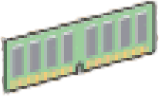
\includegraphics{./images/memoria.png}};
	\node at (1.25,0.5) {\textsc{Memoria}};
	
	\node at (3.75,1.4) {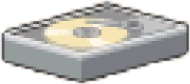
\includegraphics{./images/hdd.png}};
	\node at (3.75,0.5) {\textsc{Disco}};
	
	\node at (6.25,1.4) {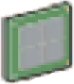
\includegraphics{./images/cpu.png}};
	\node at (6.25,0.5) {\textsc{CPU}};
	
	\node at (8.75,1.4) {
\includegraphics{./images/red.png}};
	\node at (8.75,0.5) {\textsc{Red}};
\end{tikzpicture}
}

\newcommand{\figuraSO}{
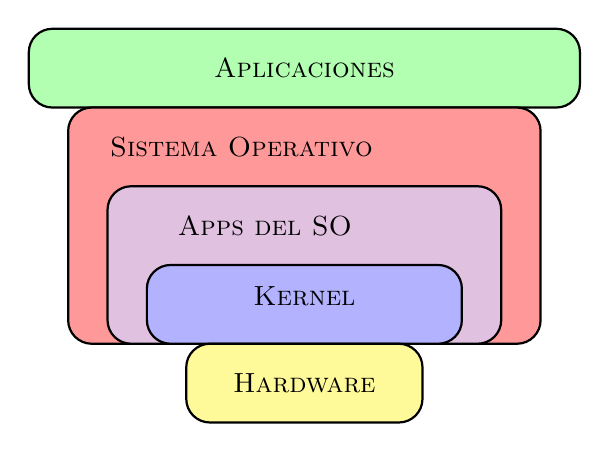
\begin{tikzpicture}
\definecolor{morado}{RGB}{177,100,177}
	\draw[rounded corners=3mm, fill=green!30, thick] (-.50,3) rectangle (6.5,4);
	\draw[rounded corners=3mm, fill=red!40, thick] (0,0) rectangle (6,3);
	\draw[rounded corners=3mm, fill=morado!40, thick] (0.5,0) rectangle (5.5,2);
	\draw[rounded corners=3mm, fill=blue!30, thick] (1,0) rectangle (5,1);
	\draw[rounded corners=3mm, fill=yellow!40, thick] (1.5,-1) rectangle (4.5,0);
	
	\node at (3,3.5) {\textsc{Aplicaciones}};
	\node at (2.2,2.5) {\textsc{Sistema Operativo}};
	\node at (2.5,1.5) {\textsc{Apps del SO}};
	\node at (3,0.6) {\textsc{Kernel}};
	\node at (3,-0.5) {\textsc{Hardware}};
\end{tikzpicture}
}

\newcommand{\figuraSOsimpl}{
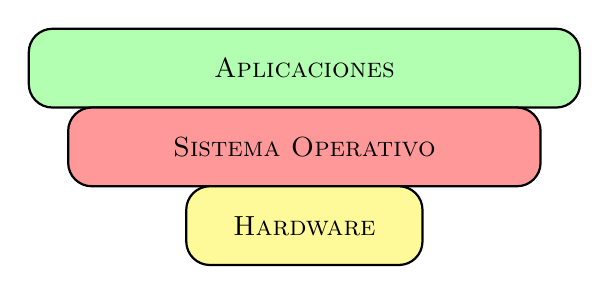
\begin{tikzpicture}
	\draw[rounded corners=3mm, fill=green!30, thick] (-0.5,1) rectangle (6.5,2);
	\draw[rounded corners=3mm, fill=red!40, thick] (0,0) rectangle (6,1);
	\draw[rounded corners=3mm, fill=yellow!40, thick] (1.5,-1) rectangle (4.5,0);
	
	\node at (3,1.5) {\textsc{Aplicaciones}};
	\node at (3,0.5) {\textsc{Sistema Operativo}};
	\node at (3,-0.5) {\textsc{Hardware}};
\end{tikzpicture}
}


\newcommand{\pizarra}{
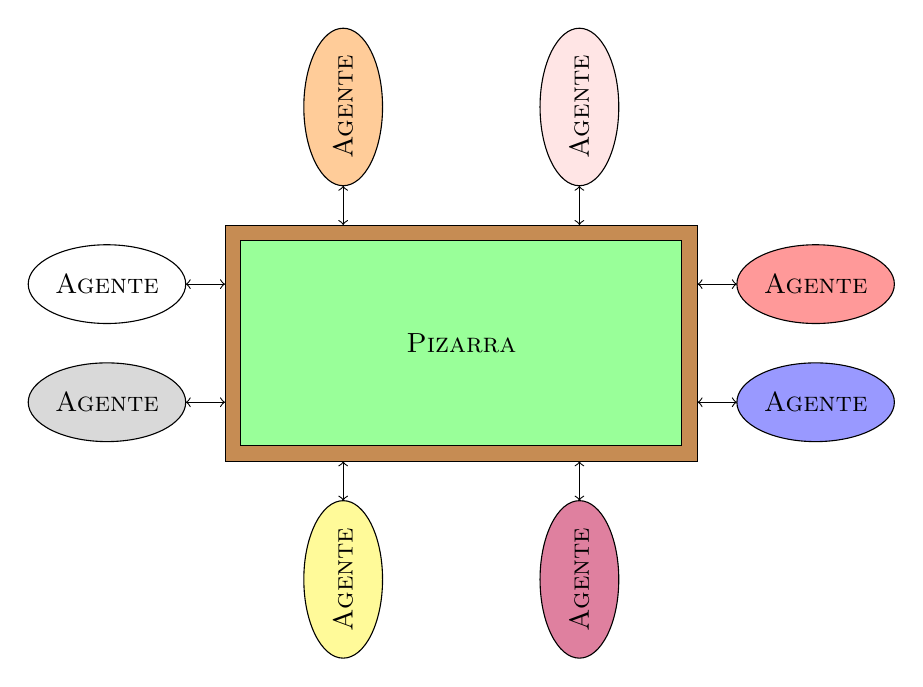
\begin{tikzpicture}
	\draw[fill=brown!90] (0,0) rectangle (6,3);
	\draw[fill=green!40] (0.2, 0.2) rectangle (5.8,2.8);
	
	\draw[fill=red!40] (7.5,2.25) ellipse (1cm and 0.5cm);
	\draw[fill=blue!40] (7.5,0.75) ellipse (1cm and 0.5cm);
	\draw[fill=yellow!40] (1.5,-1.5) ellipse (0.5cm and 1cm);
	\draw[fill=purple!50] (4.5,-1.5) ellipse (0.5cm and 1cm);
	\draw[fill=gray!30] (-1.5,0.75) ellipse (1cm and 0.5cm);
	\draw[fill=white!40] (-1.5,2.25) ellipse (1cm and 0.5cm);
	\draw[fill=orange!40] (1.5,4.5) ellipse (0.5cm and 1cm);
	\draw[fill=pink!40] (4.5,4.5) ellipse (0.5cm and 1cm);
	
	\draw[<->] (6,0.75) -- (6.5,0.75);
	\draw[<->] (6,2.25) -- (6.5,2.25);
	\draw[<->] (1.5,3) -- (1.5,3.5);
	\draw[<->] (4.5,3) -- (4.5,3.5);
	\draw[<->] (0,0.75) -- (-0.5,0.75);
	\draw[<->] (0,2.25) -- (-0.5,2.25);
	\draw[<->] (1.5,-0.5) -- (1.5,0);
	\draw[<->] (4.5,-0.5) -- (4.5,0);
	
	\node at (3,1.5) {\textsc{Pizarra}};
	\node at (7.5,2.25) {\textsc{Agente}};
	\node at (7.5,0.75) {\textsc{Agente}};
	\node[rotate=90] at (1.5,-1.5) {\textsc{Agente}};
	\node[rotate=90] at (4.5,-1.5) {\textsc{Agente}};
	\node at (-1.5,0.75) {\textsc{Agente}};
	\node at (-1.5,2.25) {\textsc{Agente}};
	\node[rotate=90] at (1.5,4.5) {\textsc{Agente}};
	\node[rotate=90] at (4.5,4.5) {\textsc{Agente}};
\end{tikzpicture}
}
